\svnInfo $Id: intro.tex 6561 2007-06-24 06:30:57Z kohlhase $
\svnKeyword $HeadURL: https://svn.omdoc.org/repos/omdoc/projects/omdoc-2.0/OpenMath-paper/intro.tex $
\section{Introduction}\label{sec:intro} 

Over the last three millennia, mathematics has developed a complicated two-dimensional
format for communicating formulae (see e.\,g.~\cite{Cajori:ahmn93,Wolfram:mnpf00} for
details). Changes in notation have been influential in shaping the way we calculate and
think about mathematical concepts, and understanding mathematical notations is an
essential part of any mathematics education.

Content Markup formats for mathematics such as {\openmath}~\cite{BusCapCar:2oms04} and
{\mathml}~\cite{CarIon:MathML03} concentrate on the functional structure of mathematical
formulae, thus allowing mathematical software systems to exchange mathematical
objects. For communication with humans, these formats rely on a ``presentation process''
(usually based on XSLT style sheets) that transforms the content objects into the usual
two-dimensional form used in mathematical books and articles.

After a conceptual analysis of the presentation process and a survey of recent approaches
to specify the notations of mathematical symbols and how to use these specifications to
transform content-oriented mathematical documents to a presentation-oriented format like
PDF or HTML, we introduce a revised specification of the presentation module of {\omdoc}
that is enabled for elisions.  We conclude by proposing how information about elisions
that a presentation algorithm performed can be included in the presentation markup and
used by a client application.

\subsection{Presentation as Composition and Elision}

Many such presentation processes have been proposed, and all have their strengths and
weaknesses. In this paper, we conceptualize the presentation of mathematical formulae as
consisting of two components: the two-dimensional {\defemph{composition}} of visual
sub-presentations to larger ones and the {\defemph{elision}} of formula parts that can be
deduced from context.

Most current presentation processes concentrate on the relatively well-understood
composition aspect and implement only rather simple bracket elision algorithms. But the
visual renderings of formulae in mathematical practice are not simple direct compositions
of the concepts involved: mathematicians gloss over parts of the formulae, e.\,g.\ leaving
out arguments, iff they are non-essential, conventionalized or can be deduced from the
context. Indeed this is part of what makes mathematics so hard to read for beginners, but
also what makes mathematical language so efficient for the initiates. A common example is
the use of $\log(x)$ or even $\log x$ for $\log_{10}(x)$ or similarly $\lden t\rden$ for
$\lden t\rden_{\cal M}^\phi$, if there is only one model $\cal M$ in the context and
$\phi$ is the most salient variable assignment. Another example are the bracket elision
rules in arithmetical expressions: $ax+y$ is actually $(ax)+y$, since multiplication
``binds stronger'' than addition. Note that we would not consider the ``invisible times''
operation as another elision, but as an alternative presentation. Finally, there are
extreme examples of elision or substitution like Church's dot notation, where a dot stands
for a left bracket, whose mate is as far to the right as consistent with the remaining
(un-elided) brackets. For instance $(a\cdot.\,b+c)-d$ stands for $(a\cdot(b+c))-d$, and
$\forall x,y.\phi\wedge\psi$ stands for $\forall x,y (\phi\wedge\psi)$.

Now that we have convinced ourselves that the elision is an important component of
generating high-quality presentations, let us reconsider the presentation process itself
to see how composition and elision interact.

We will start from the observation that in content markup formalisms for mathematics
formulae are represented as ``formula trees''. Concretely, we will concentrate on
{\openmath} objects, the conceptual data model of {\openmath} representations, since it is
sufficiently general, and work is currently under way to re-engineer content {\mathml}
representations based on this model. Furthermore, we observe that the target of the
presentation process is also a tree expression: a layout tree made of layout primitives
and glyphs, e.\,g.\ a presentation {\mathml} expression. If we make examples with
{\TeX/\LaTeX} it is only since it is universally understood; here, the layout tree is the
parse tree implicit in the linear {\TeX/\LaTeX} string. This notwithstanding, we finally
observe that even though formula presentations are two-dimensional in principle, large
parts are more or less linear, and therefore mathematical notation relies on brackets to
allow the reader to reconstruct the content structure from the presentation.

\subsection{Characteristics of Mathematical Symbols}\label{sec:characteristics}

In a nutshell, {\openmath} objects are trees built up from {\defemph{variables}} and
{\defemph{symbols}} at the leaves and {\defemph{applications}} and {\defemph{binders}} as internal
nodes. 

\begin{wrapfigure}{r}{3cm}\vspace*{-.5em}
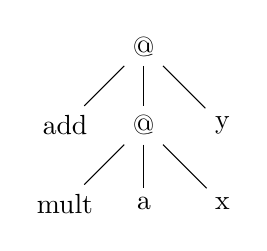
\begin{tikzpicture} 
\node (top) at (1,2) {@};
\node (plus) at (0,1) {add};
\node (mid) at (1,1) {@};
\node (y) at (2,1) {y};
\node (mult) at (0,0) {mult};
\node (a) at (1,0) {a};
\node (x) at (2,0) {x};
\draw(top) -- (plus);
\draw(top) -- (mid);
\draw(top) -- (y);
\draw(mid) -- (mult);
\draw(mid) -- (a);
\draw(mid) -- (x);
\end{tikzpicture}\vspace*{-.5em}
\end{wrapfigure}
For our purposes, symbols and applications are the most important concepts,
therefore let us fortify our intuition with the example on the right: the sum $ax+y$ above
would be represented by a tree with an application at the root, whose first child is the
symbol\footnote{Note that a symbol is not a glyph --- these are often confused, the symbol
  here stands for the mathematical concept of a sum, not the glyph $+$.} for addition, the
third child is the variable with the name $y$, and the second child is another application
whose children are the symbol for multiplication and the variables with names $a$ and $x$.

As part of the functional notation of mathematics popularized by Leibniz and Newton for
algebra, the visual appearance of a subformula was largely determined by its head
operator, which nowadays carries much of the notational conventions, which are usually
phrased in terms of the following notational characteristics of a symbol:

\begin{description}
\item[fixity (for operators):] Is the operator displayed as a prefix (like a function
  symbol), as a postfix (like the factorial symbol $!$) or as an infix (like most
  arithmetic operators)?  Operators of higher arity can also have a ``mixfix'' style;
  consider the 4-ary typing judgment operator $\Gamma\vdash_\Sigma t\colon\alpha$, which
  states that a term $t$ has type $\alpha$ in a variable context $\Gamma$ and a signature
  $\Sigma$.
\item[left and right brackets:] If an operation is bracketed, are round, square, curly,
  angle, or other brackets used? In fact brackets in mathematical vernacular are mostly
  round brackets; technical notations sometimes use others, e.g. {\mathematica} uses
  square ones throughout. Note that not all parts of a presentation that look like
  brackets are indeed. For instance in a half-open interval as $]a;b]$, is actually mixfix
  operator where the bracket-like glyphs ``$]$'' look and conventionally stretch like
  brackets, but do not match and cannot be elided like brackets. They are easy to mistake
  for brackets, since they (as all fully inhabited mixfix presentations) make brackets for
  the arguments unnecessary. We would consider it a semantic anomaly to present an
  ``interval'' operator as an infix ``;'' with obligatory left and right brackets ``$]$''
  and ``$]$''.
\item[precedence (for operators):] If an operation $O$ with a high precedence occurs as an
  argument of an operator with a lower precedence, the brackets around $O$ can be
  elided.
\item[associativity (for infix operators):] To elide brackets for $n$-ary operators
  ($n>2$), it must be known whether they are associative (i.\,e.\ $(a\circ b)\circ c =
  a\circ(b\circ c) =: a\circ b\circ c$) or obey ``left-associative'' or
  ``right-associative'' elision conventions (e.g.
  $\alpha\to\beta\to\gamma:=\alpha\to(\beta\to\gamma)$ for right-associative function
  types).
\end{description}
The first two characteristics specify the composition of the visual representations,
whereas the latter two are concerned with bracket elision. Furthermore, the {\bf{role}} of
a symbol in the formula context needs to be taken into account: Is it a simple
{\emph{constant}} like $\mathbb{R}$, a {\emph{function}} that is applied to arguments, or
a {\emph{binder}} that binds variables like $\forall x.p(x)$. This is most pronounced for
functions that can occur either applied to arguments or as the concept alone.
Presentations differ for these occasions, e.g. for the absolute value function, we write
something like $\bigl|\cdot\bigr|$ with a ``dummy argument'' $\cdot$ when it is not in an
applied context.

\subsection{Notation Definitions}\label{sec:notdef}

Mathematical formulae given in the XML-based structural formats {\openmath} and Content
{\mathml} are commonly presented by implementing one XSLT template~\cite{W3C:xslt2} per
symbol, which specifies how to transform this symbol to the output format---another XML
format like Presentation {\mathml}, or a non-XML format like {\TeX}, for example.
Appropriate templates for the arguments are usually applied recursively.

The following listing shows a straightforward way to transform the exponentiation operator
from {\openmath} to {\TeX}:
 
\begin{lstlisting}[language=XSLT,caption=An XSLT presentation template,label=lst:template]
 <xsl:template match="om:OMA[om:OMS[@cd='arith1' and @name='power']]">
   <xsl:apply-templates select="*[2]"/> <!-- first argument -->
   <xsl:text>^{</xsl:text>
   <xsl:apply-templates select="*[3]"/> <!-- second argument -->
   <xsl:text>}</xsl:text>
 </xsl:template>
\end{lstlisting}

To save authors from the tedious and error-prone task of writing similar templates for
every symbol and notation variant, different facilitations have been invented. The
probably earliest examples were the presentation architecture in
{\omdocv{1.0}}~\cite{Kohlhase:otormd00} and Naylor's\&Watt's {\openmath}
conversion~\cite{Naylor:conversion}. Both supply XML-based {\defemph{notation
    definitions}} that can be transformed into a suitable XSLT conversion style sheet by a
meta-stylesheet.

In {\omdoc}, a template like the one above would be generated from a
{\element{presentation}} element of the form
\begin{lstlisting}[mathescape]
<presentation for="power" theory="arith1" role="application" class="1">
  <style format="TeX">
    <recurse select="*[2]"/><text>^{</text><recurse select="*[3]"/><text>}</text>
  </style>
  $\ldots$
<presentation>
\end{lstlisting}
where the {\attribute[ns-elt=xsl]{match}{template}} attribute is generated from the
attributes on the {\element{presentation}} element and the contents from the ones on the
{\element{use}} element. In contrast to this, where notations definitions are thought as
directed rules from content to presentation, Naylor's\&Watt's framework views them as
equivalences between representations. For the example above we would have
\begin{lstlisting}[mathescape,language=XML,morekeywords={Notation,version,semantic-template},
caption=A Template-Based Notation Definition,label=lst:template-based]
<Notation>
  <version style="1">
    <tex>\arg{a1}{n}^{\arg{a2}{m}}</tex>
    $\ldots$
  </version>
  <semantic-template>
    <OMA><OMS cd="power" name="arith1"/>
      <OMV name="n" id="a1/>
      <OMV name="n" id="a2/>
    </OMA>
  </semantic-template>
</Notation>
\end{lstlisting}
We will call the first approach to notation specification {\defemph{symbol-based}}, as the
notation is tied to a concrete symbol, and the second one {\defemph{template-based}}. Note
that the template-based approach is in principle more directly invertible (e.g. for
parsing), and more expressive (it would e.g. allow to present $log(e,x)$ as $\ln(x)$ and
$log(b,x)$ as $\log_b(x)$). But this has not been realized in practice, since the
presentation of mathematical formulae {\emph{is indeed}} tied to symbols, so all templates
are indeed one-level like the one in the example above. On this fragment, both approaches
are equivalent. Note furthermore that many of the notational characteristics of a symbol
mentioned in section~\ref{sec:characteristics} actually do not belong to the symbol but to
its presentation. For example, the division operator, presented as $\cdot/\cdot$, has a
higher precedence than $\frac{\;\cdot\;}{\;\cdot\;}$---consider $1/(a+b)$ vs.\
$\frac{1}{a+b}$.

In {\omdocv{1.2}}~\cite{Kohlhase:omdoc1.2}, all of these characteristics can be specified
as attributes to one out of potentially multiple {\element{presentation}} elements that
refer to a {\element{symbol}}. For some aspects like mix-fixity, this declarative syntax
is not yet expressive enough; in this case, embedded XSLT templates must be used, losing
declarativity. In this paper, we rethink the notation definition system and propose a
declarative system extending ideas from the notation definition system in the {\isabelle}
theorem proving environment~\cite{Paulson:Isabelle05}.

%%% Local Variables: 
%%% mode: stex
%%% TeX-master: "presel"
%%% fill-column: 90
%%% sentence-end-double-space: nil
%%% End: 

% LocalWords:  mult xsl om OMA OMS cd arith Naylor's Watt's mathescape ns elt
% LocalWords:  tex OMV presel
